\section{The Physics of Nuclear Interactions}

This section provides the physical background needed to understand the probabilities of neutron interactions with matter. Due to the very large neutron densities on the order of \(10^8\) per cm$^3$, neutron interactions with matter will only be regarded in an average sense, as such detailed accounting of every neutron is unneccessary. 

\subsection{Radioactive Decay}
\label{sec:RadioactiveDecay}
There are four important types of radioactive decay:

\begin{enumerate}
\item Alpha decay - a nucleus emits a helium nucleus,
\item Beta decay - a neutron is converted to a proton in the nucleus, and an electron and neutrino are emitted,
\item Gamma decay - a nucleus transitions from a higher energy state to a lower energy state and in the process emits a photon, and
\item Neutron decay - a neutron is emitted
\end{enumerate}

The physics of radioactive decay are based on the assumption that the probability of decay of a nuclide is constant in time - an excellent approximation. This probability of decay per unit time, \(\lambda\) is known as the decay constant. If the probability of decay is a constant independent of the number of nuclei present or other environmental conditions, the rate of the change of the number of nuclei \(N\) is proportional to the number present:

\beq
\label{eq:Decay}
\frac{dN(t)}{dt}=-\lambda N(t)
\eeq

The quantity \(\lambda N\) represents the instantaneous number of radioactive decays occurring, and is also referred to as the activity \(A\):

\beq
\label{eq:ActivityDef}
A(t)\equiv\lambda N(t)
\eeq

Activity is typically quoted in units of Curies, or \(3.7\times10^{10}\) decays per second, roughly equivalent to the activity of one gram of radium. Solution of Eq. \eqref{eq:Decay} provides an expression for the number of nuclei present given an initial number \(N_0\):

\beq
\label{eq:DecayEqn}
N(t)=N_0e^{-\lambda t}
\eeq

Note that for systems of different nuclides, a system of equations of the form in Eq. \eqref{eq:Decay} exists with additional source terms representing decay chain effects; this constant-coefficient system can be easily solved. The instantaneous rate of radioactive decay is obtained simply by multiplying \(N(t)\) by the decay constant, from which it is clear that the probability a nuclei will decay in a time interval \(t\) to \(t+dt\) is:

\beq
\label{eq:ProbabilityDecay}
p_{\text{decay}}=\lambda e^{-\lambda t}dt
\eeq

The expectation value of the lifetime \(\bar{t}\) of a nuclide is calculated by computing the first moment of the probability of decay:

\beqa
\label{eq:MeanLifetime}
\bar{t}\equiv&\int_0^\infty dt\ t\lambda e^{-\lambda t}dt\\
=&\frac{1}{\lambda}
\eeqa

Eq. \eqref{eq:MeanLifetime} can be more intuitively understood if the probability of decay were a delta function for a specific time \(t_i\), in which case the integral in Eq. \eqref{eq:MeanLifetime} would simply equal \(t_i\), as expected. For gamma decay, a nucleus transition between two states with a difference in energies \(\Delta E\). From the Heisenberg uncertainty principle, if \(\Delta t\) is taken as the average lifetime of the higher-energy state before decaying to the lower-energy state, it is clear that \(\Delta E\propto\lambda\), so states with very large transitions in energy tend to have much larger decay constants than smaller-energy transitions.

\subsection{Nuclear Collisions}
As opposed to radioactive decay discussed in Section \ref{sec:RadioactiveDecay}, the probabilities of nuclear collisions are not constants independent of all environmental factors. For nuclear collisions, the probability of interaction is dependent on both the identities of the two interacting particles and their relative velocity (which accounts for both their relative energy and directions of motion). All nuclear reactions are accompanied by the absorption or release of energy; this energy can be computed based on the mass \(m\) that is converted to energy and vice versa using the following result from general relativity:

\beq
E=mc^2
\eeq


%Additional collisions of importance include \((n,\alpha)\) reactions, common in absorber materials introduced for reactor control. 

The microscopic cross section \(\sigma\) is the fundamental property data required for the analysis of nuclear systems. The microscopic cross section for reaction \(i\), \(\sigma_i\), is {\it proportional} to the probability that a neutron will interact with a specific nucleus through a reaction of type \(i\). More specifically, the microscopic cross section is the probability per nucleus in a target of unit cross-sectional area that a neutron in a beam of intensity \(I\) will interact with it. While not {\it equivalent} to the effective area presented by the target nuclei to a beam, typical units of \(\sigma\) do roughly correspond to the cross sectional area of a nucleus represented as a circle with nuclear radius of \(10^{-12}\) cm. The total cross section is the sum of the scattering and absorption cross sections. While neutrons are released in fission such that it could in some sense be treated as a scattering reaction, fission is customarily treated as an absorption interaction.

The microscopic cross section only indicates the probability of interaction with a single nucleus in a target of unit cross-sectional area. To obtain the probability of interaction per unit distance traveled by the particle, \(\sigma\) must be multiplied by the number density \(N\) of the target material. The macroscopic cross section for reaction \(i\), \(\Sigma_i\), is defined as the probability of interaction per unit travel of a particle with {\it any} nucleus:

\beq
\label{eq:MacroscopicSigmaDef}
\Sigma_i\equiv\sigma_iN
\eeq

Similar to the definition for the probability of decay in Eq. \eqref{eq:ProbabilityDecay}, the probability that a neutron has its first interaction in the spatial interval \(x\) to \(x+dx\) is simply the multiplication of the interaction probability per unit distance with the instantaneous local value of the beam intensity (obtained from a differential equation with solution identical to Eq. \eqref{eq:DecayEqn}):

\beq
p_{\text{interaction}}=\Sigma_te^{-\Sigma_tx}dx
\eeq

The expectation value of the distance traveled before interacting \(\bar{x}\) is calculated by computing the first moment of the probability of interaction:

\beqa
\bar{x}\equiv&\int_0^\infty dx\ x\Sigma_te^{-\Sigma tx}\\
=&\ \frac{1}{\Sigma _t}
\eeqa

The average distance traveled between interactions, \(\bar{x}\) is commonly referred to as the mean free path. The macroscopic cross section represents the probability per unit path length traveled that a particle undergoes an interaction; multiplication by the velocity of the particle gives the frequency with which such interactions occur. This reaction frequency for interaction type \(i\) in nuclide \(i\) is often referred to as the ``reaction rate frequency:''

\beq
\label{eq:ReactionRateFrequency}
\text{Reaction rate frequency}\equiv \|\vv{v}-\vv{V}\|\sigma_i(\|\vv{v}-\vv{V}\|)N_j
\eeq

where \(\vv{v}\) is the neutron velocity and \(\vv{V}\) the velocity of the colliding nucleus. Intuitively, the reaction rate and microscopic cross section must be proportional to the {\it relative} velocity. Eq. \eqref{eq:ReactionRateFrequency} is written in terms of \(v\), rather than the relative velocity, through the use of thermally-average cross sections described in Section \ref{sec:ThermalNeutrons}. By a similar procedure as performed to obtain the average lifetime and path length, the average time between collisions can be calculated as \(1/(v\Sigma)\).\

For all reaction types except potential scattering, described in Section \ref{sec:PotentialScattering}, the incident neutron interacts with the nuclear potential of the target nuclide to form a compound nucleus. A compound nucleus is inferred to exist due to the relatively long times observed between interaction with a neutron and subsequent release of reaction products. During this lifetime of the compound nucleus, energy is transferred from the neutron to the nucleons, which after some time leads to the collapse of the compound nucleus. The relatively long lifetime of the compound nucleus makes it very likely that the reaction products are independent of the initial state of the neutron, and only dependent on the state of the compound nucleus. 

The formation of a compound nucleus is a type of resonance reaction; the total energy available to be transferred to the compound nucleus is the sum of the energy in the \gls{cm} frame and the additional \gls{be} of the neutron. When this total available energy very closely matches an energy state of the compound nucleus, formation is much more likely to occur, leading to resonance structures in cross sections related to reactions involving compound nucleus formation. Because the formation of the compound nucleus leads to some degree of independence of the reaction products on the initial state of the neutron, the energy dependence of the cross sections for many different reactions share common features. 

The neutron wavelength \(\lambda_n\) is proportional to \(1/\sqrt{E}\), and is important in understanding several of the energy ranges of cross section behavior:

\beq
\label{eq:NeutronWavelength}
\lambda_n=\frac{h}{\sqrt{2mE}}
\eeq

where \(h\) is the Planck constant and \(\sqrt{2mE}\) is the momentum of the neutron. There are generally four regions of unique behavior in the total scattering cross section for {\it light} nuclei, bounded by the approximate energy ranges:

\begin{itemize}
\item \(10^{-4}-10^{-2}\) eV - the neutron wavelength becomes on the order of the spacing between atoms, and a neutron interacts with groups of nuclei simultaneously. If the target material is organized in a lattice, the neutron is diffracted, and a sensitive energy dependence exists as the neutron energy approaches multiples of the interatomic spacing between different ``views'' of the lattice. Thresholds for this type of interaction typically occur at \(10^{-3}\) eV and above. Throughout this {\it entire} energy range, the neutron energy may be lower than the chemical binding energy of the material, in which case the neutron interacts with the material as an aggregate quantity. The neutron no longer interacts with a free atom, but rather may excite lattice vibrations or rotate atoms in a lattice. The thermal motion of the target nuclei is important; neutron energies comparable to the thermal energy of the material cannot be analyzed without considering the thermal motion of the target. In this energy range, the cross section has a \(1/\sqrt{E}\) dependence, with diffraction effects superimposed and leading to a rather large increase in the total cross section at around \(10^{-3}\) once the diffraction cutoff is reached.
\item \(10^{-2}-10^6\) eV - the \(\sigma_s\) is dominated by potential scattering; because \(\sigma_p\) is approximately independent of energy, this gives a nearly constant \(\sigma_s\) 
\item \(10^6-10^7\) eV - resonance region; large peaks are observed where \(E_c+E_b\) coincides with an excited state of the compound nucleus
\item Above \(10^7\) eV - fast spectrum region, characterized by a rapid decrease in the total cross section as the neutron wavelength decreases according to Eq. \eqref{eq:NeutronWavelength} until it is sufficiently small that interaction with any nucleus becomes highly improbable.
\end{itemize}

For light nuclei, the lowest-lying resonance energy states are in the MeV range, while for heavy nuclei begin in the eV to keV range, and the resonance region extends down to a lower energy range.

For light nuclei with \(A<25\), the epithermal and fast energy ranges are dominated by separated resonances; there is no \gls{urr} in light nuclei. Epithermal and low energies are dominated by potential scattering. For intermediate and heavy nuclei, high energies are characterized by inelastic scattering, overlapping resonances, and continuum resonances. Intermediate energies are characterized by radiative capture and elastic scattering, while low energies are dominated by potential scattering for intermediate nuclei and radiative capture for heavy nuclei.

Resonance effects are most significant in heavy nuclides. At high energies, the energy states in heavy nuclides become closer and closer to one another, forming a very complicated resolved resonance structure that eventually overlaps so significantly to be considered the \gls{urr} with an onset typically in the range of 1 to 10 keV.

%At thermal energies, carbon is nearly a pure scatterer - the scattering cross section is approximately three orders of magnitude larger than the absorption cross section, and will therefore undergo approximately \(10^3\) scattering reactions before being absorbed. For a scattering cross section of 4.8 barns, this gives a mean free path of thermal neutrons in graphite of approximately 2.6 cm.

Cross section data, especially for resonances, tends to be stored as a function of several fitting parameters rather than cross sections tabulated at discrete energies in order to reduce the required storage. Processing codes such as NJOY then convert the cross section data to a useable form for computational activities. 

\subsubsection{Radiative Capture}

The radiative capture cross section \(\sigma_\gamma\) exhibits strong resonance structure, since absorption of a neutron leads to the formation of a compound nucleus that decays by transitioning between different energy states through the release of a cascade of photons. Radiative capture is an important interaction due to its removal of neutrons from the fission chain reaction. As temperatures increase, radiative capture resonances broaden, resulting in increased radiative capture reaction rates in nuclides such as U-238, which in most reactor designs leads to negative reactivity feedback. Radiative capture is also the primary mechanism by which U-238 is transmuted to Pu-239.

U-238 has several low-lying resonances in the eV range, with the lowest resonance at 6.67 eV with a narrow width of 0.027 eV and a peak of \(7\times10^3\) barns that is about four orders of magnitude larger than the nearby cross section. For resonances that are widely separated from one another such as to not overlap, the energy dependence of \(\sigma_\gamma\) can be approximated using the Breit-Wigner single-level resonance formula:

\beq
\label{eq:BW}
\sigma_\gamma(E_c)=\sigma_0\frac{\Gamma_\gamma}{\Gamma}\sqrt{\frac{E_0}{E_c}}\left\lbrack1+4\left(\frac{E_c-E_0}{\Gamma}\right)^2\right\rbrack^{-1}
\eeq

where \(E_0\) is the energy on which the resonance is centered, \(\Gamma\) is the total line width of the resonance, which captures the width of the energy level at the \gls{fwhm}, and \(\Gamma_\gamma\) is the radiative line width that captures the probability that the compound nucleus decays via the emission of a photon. \(\sigma_0\) is the total cross section at \(E_0\) which scales as:

\beq
\sigma_0\propto\frac{(A+1)^2}{A^2E_0}\sqrt{E}
\eeq

but also depends on other factors such as spin. Because resonance effects are most significant in heavy nuclei, \(E_c\) is well-approximated by \(E\). Radiative capture cross sections tend to be largest at low energies, and generally decrease continuously with energy except for the presence of resonances. For low energies, \(\sigma_\gamma\propto1/\sqrt{E}\), while at higher energies falls off very quickly with energy as \(\sigma_\gamma\propto1/\sqrt{E^5}\).

Radiative capture in U-238 and Th-232 produce fissile isotopes through the following decay chains:

\beq
U-238 + n\rightarrow U-239\rightarrow Np-239\rightarrow Pu-239
\eeq

\beq
Th-232+n\rightarrow Th-233\rightarrow Pa-233\rightarrow U-233
\eeq

For such breeding isotopes to be possible, the number of neutrons produced per neutron absorbed by a material, defined as \(\eta\), must exceed unity. 

\beqa
\label{eq:Eta2Def}
\eta\equiv&\frac{\text{average number of neutrons produced}}{\text{average number of neutrons absorbed}}\\
\equiv&\frac{\sum_{i=1}^N\nu_i\Sigma_{f,i}}{\sum_{i=1}^N\Sigma_{a,i}}
\eeqa

where \(N\) is the total number of types of fissile isotopes present in the fuel mixture. \(\eta\) is slightly greater than two in the thermal and epithermal range, but dramatically increases above 10 keV where the capture-to-fission ratio dramatically decreases, indicating the onset of an energy range in which breeding is more easily achievable. In the fast energy range, \(\eta\) is largest for Pu-239 and Pu-241. Breeding in the thermal spectrum is only possible with U-233, which has an \(\eta\) of about 2.4. 

\subsubsection{Fission Reactions}

Similar to radiative capture, fission is the result of compound nucleus formation, and therefore the fission resonance structure for fissile nuclides shares similarities with the radiative capture resonance structure. However, for nuclei that only undergo fast fission such as U-238 and Th-232, the fission cross section is essentially zero until reaching the MeV range, where cross sections become on the order of 1 barn.

\subsubsection{Potential Scattering Reactions}
\label{sec:PotentialScattering}

In a potential scattering reaction, two colliding bodies interact as hard spheres without forming a compound nucleus. There is very weak energy dependence in potential scattering, and the cross section is often well-approximated by the cross-sectional area of the target nuclide nucleus for intermediate energies. The radius of a nucleus for a nuclide with mass number \(A\) can be approximated as:

\beq
R\ (\text{cm})\approx1.25\times10^{-13}A^{1/3}
\eeq

For U-235, \(\sigma_p\approx7.5 barns\). The energy and angle dependence of the double differential potential scattering cross section can be determined analytically using conservation of momentum and energy for scattering from stationary low \(A\) nuclides and neutron energies less than 1 MeV. The potential scattering cross section can be decomposed into a probability of interaction at energy \(E\) multiplied by the probably of an incoming energy and angle \(E\) and \(\hO\) being scattered to an outgoing energy and angle \(E'\) and \(\hO\):

\beq
\label{eq:DifferentialSigma}
\sigma_p(E\rightarrow E',\hO\rightarrow\hO')=\sigma_p(E)P(E'\rightarrow E)P(\hO\rightarrow\hO')
\eeq


\subsubsubsection{Scattering Off Stationary Nuclei}
\label{sec:PotentialStationary}
For potential scattering off stationary nuclei, these two probabilities can be calculated as follows. It will be useful to transform the coordinate system to the \gls{cm} frame. The velocity of the center of mass frame \(\vv{\mathscr{V}}\) is calculated as the mass-weighted velocities in the lab frame:

\beq
\label{eq:CMVelocity}
\vv{\mathscr{V}}\equiv\frac{m\vv{v}+M\cancel{\vv{V}}}{m+M}
\eeq

where \(m\) is used to represent the neutron mass and \(M\) the target nuclide mass, with \(\vv{v}\) representing the neutron velocity and \(\vv{V}\) the target nuclide velocity. Without a \(CM\) subscript, all quantities are inferred to represent the lab-frame quantities. In this analysis, it is assumed that the target nucleus is stationary in the lab frame such that \(\vv{V}=0\). The velocities in the \gls{cm} frame of the neutron and target nucleus are:

\beqa
\label{eq:CMVelocities}
\vv{v}_{CM}=&\vv{v}-\vv{\mathscr{V}}\\
=&\frac{M/m}{1+M/m}\vv{v}
\eeqa

\beqa
\label{eq:CMVelocities2}
\vv{V}_{CM}=&\cancel{\vv{V}}-\vv{\mathscr{V}}\\
=&\frac{1}{1+M/m}\vv{v}
\eeqa

where Eq. \eqref{eq:CMVelocity} was used for \(\vv{\mathscr{V}}\). The total momentum in the \gls{cm} frame is obtained by multiplying masses with the velocities in the \gls{cm} frame in Eqs. \eqref{eq:CMVelocities} and \eqref{eq:CMVelocities2} and summing, which will show that the total momentum in the \gls{cm} frame is zero (which is also the {\it definition} of the \gls{cm} frame). The kinetic energies in the lab and \gls{cm} frame are:

\beq
\label{eq:ELab}
E=\frac{1}{2}\left(m\|\vv{v}\|^2+M\cancel{\|\vv{V}\|^2}\right)
\eeq

\beqa
\label{eq:ECM}
E_{CM}=&\frac{1}{2}\left(m\|\vv{v}_{CM}\|^2+M\|\vv{V}_{CM}\|^2\right)\\
=&\frac{1}{2}\frac{Mm}{M+m}\|\vv{v}\|^2
\eeqa

The energies in the lab and \gls{cm} are related through Eqs. \eqref{eq:ELab} and \eqref{eq:ECM} as:

\beq
E_{CM}=\frac{M}{M+m}E
\eeq

from which it can be seen that the energy in the \gls{cm} is always less than the energy in the lab frame because some energy is allocated to the movement of the \gls{cm} frame itself via \(\vv{\mathscr{V}}\). Using conservation of momentum and energy, it can be shown that the velocity magnitudes of the projectile and target following the collision in the \gls{cm} frame remain constant - only the velocity vectors are rotated through an angle \(\theta_c\) in the \gls{cm} frame. Rearranging Eq. \eqref{eq:CMVelocities} and defining \(\theta\) as the lab frame scattering angle, two relationships can be written:
% derivation showing that velocity magnitudes remain constant in CM frame pre- and post-collision is missing

\begin{subequations}
\label{eq:CMvsLab}
\begin{eqnarray}
v'\sin{(\theta)}&=&v'_{CM}\sin{(\theta_c)}\\
v'\cos{(\theta)}&=&v'_{CM}\cos{(\theta_c)}+\mathscr{V}
\end{eqnarray}
\end{subequations}


\begin{tcolorbox}[breakable]
Dividing Eq. \eqref{eq:CMvsLab}a by Eq. \eqref{eq:CMvsLab}b gives the relationship between the lab and \gls{cm} frame scattering angles:

\beq
\label{eq:CMtoLab}
\tan{(\theta)}=\frac{\sin{(\theta_c)}}{m/M+\cos{(\theta_c)}}
\eeq

Cross sections are typically measured in the \gls{cm} and utilized computationally in the lab frame, so Eq. \eqref{eq:CMtoLab} is useful for transforming measured angular-dependent cross sections to the lab frame. Eq. \eqref{eq:CMtoLab} only represents a transformation of the scattering angles - to transform the angular differential cross sections, write such cross sections in differential form using the \(\theta\) component of the solid angle differential in Eq. \eqref{eq:DifferentialOmega}:

\beq
\sigma\sin{(\theta)}d\theta=\sigma_{CM}\sin{(\theta_{CM})}d\theta_{CM}
\eeq

which gives the following relationship between the lab and \gls{cm} angular differential cross sections:

\beq
\sigma(\theta)=\sigma_{CM}(\theta_{CM})\frac{\left\lbrack\frac{m^2}{M^2}+\frac{2m}{M}\cos{(\theta_{CM})}+1\right\rbrack^{3/2}}{1+\frac{m}{M}\cos{(\theta_{CM})}}
\eeq
% derivation missing
\end{tcolorbox}

Applying the law of cosines between the triangle formed by \(\vv{v}_{CM}'\), \(\vv{v}'\), and \(\vv{\mathscr{V}}\) gives:

\beqa
\label{eq:FinalVelocity}
(v')^2=&\ (v'_{CM})^2+\mathscr{V}^2-2v'_{CM}\mathscr{V}\cos{(\pi-\theta_{CM})}\\
=&\ \frac{M^2/m^2+1+2M/m\cos{(\theta_{CM})}}{(1+M/m)^2}v^2\\
\eeqa

where Eqs. \eqref{eq:CMVelocities} and \eqref{eq:CMVelocities2} have been used along with the identity \(\cos{(\pi-x)}\equiv-\cos{(x)}\). Because kinetic energy is proportional to \(v^2\), and masses do not change during an elastic scattering collision, Eq. \eqref{eq:FinalVelocity} can equivalently be written in terms of the initial and final energies:

\beqa
\label{eq:ElasticScatE}
\frac{E'}{E}=&\ \frac{M^2/m^2+1+2M/m\cos{(\theta_{CM})}}{(1+M/m)^2}\\
=&\ \frac{1}{2}\left\lbrack(1+\alpha)+(1-\alpha)\cos{(\theta_{CM})}\right\rbrack\\
\eeqa

where \(\alpha\) is defined as:

\beq
\alpha\equiv\left(\frac{M/m-1}{M/m+1}\right)^2
\eeq

Eq. \eqref{eq:ElasticScatE} shows that there is a one-to-one relationship between the energy transfer in elastic scattering off stationary nuclei and the \gls{cm} scattering angle. Eq. \eqref{eq:ElasticScatE} also shows that, for a given value of \(\alpha\), \(\theta_{CM}=0\) corresponds to the minimum energy loss (a ``miss'') and \(\theta_{CM}=1\) to the maximum energy loss (backscattering). For a given value of \(\alpha\), the maximum energy loss in a single collision therefore corresponds to backscattering, for which Eq. \eqref{eq:ElasticScatE} gives \(E'=\alpha E\). Therefore, to lose the maximum amount of energy, \((1-\alpha)E\), in a single collision, \(\alpha\) should be small, which occurs for small \(M/m\), or very light nuclei. Table \ref{table:FractionalEnergyLoss} shows the maximum fractional energy loss normalized by \(E\) for elastic scattering off stationary nuclei, where \(M/m\) is approximated as \(A\); as can be seen, lighter nuclides are dramatically more effective thermalizers.

\begin{table}[H]
\caption{Maximum fractional energy loss normalized by \(E\) for elastic scattering off stationary nuclei for several common nuclei.}
\centering
\begin{tabular}{c c c}
\hline\hline
Nuclide & \(\alpha\) & Fractional Energy Loss\\ [0.5ex]
\hline
H-1 & 0.00 & 1.00\\
H-2 & 0.11 & 0.89\\
C-12 & 0.72 & 0.28\\
U-235 & 0.98 & 0.02\\
\hline
\end{tabular}
\label{table:FractionalEnergyLoss}
\end{table}

Because there is a one-to-one relationship between the energy loss and scattering angle in the \gls{cm} frame, we can postulate that there is similarly a one-to-one relationship between \(P(E\rightarrow E')\) and \(P(\hO_{CM}\rightarrow\hO_{CM}')\). The probability of scattering from \(\hO_{CM}\) to \(\hO'_{CM}\) multiplied by the total scattering cross section, is simply equal to the differential scattering cross section according to Eq. \eqref{eq:DifferentialSigma}:

\beq
\sigma_sP(\hO_{CM}\rightarrow\hO'_{CM})d\hO'_{CM}=\sigma_{CM}(\theta_{CM})2\pi\sin{(\theta_{CM})}d\theta_{CM}
\eeq

where the scattering is assumed azimuthally symmetric such that \(\sigma_{CM}\) can be written as a function of a single scattering angle \(\theta_{CM}\). Assuming this one-to-one relationship gives:

\beq
\label{eq:OnetoOneEHO}
P(E\rightarrow E')dE'=-\frac{\sigma_{CM}(\theta_{CM})}{\sigma_s}2\pi\sin{(\theta_{CM})}d\theta_{CM}\\
\eeq
% don't know why the RHS is negative

Differentiating Eq. \eqref{eq:ElasticScatE} to obtain \(dE'\) and plugging into \eqref{eq:OnetoOneEHO} gives the differential energy component of the elastic scattering cross section:

\beq
\label{eq:ScatteringDifferentialProb}
P(E\rightarrow E')=\begin{cases}\frac{4\pi\sigma_{CM}(\theta_{CM})}{(1-\alpha)E\sigma_s} & \alpha E\leq E'\leq E\\
0 & else
\end{cases}
\eeq

For light nuclei and energies less than about 10 MeV, \(\sigma_{CM}\) is isotropic such that:

\beq
\label{eq:IsotropicSigmaCM}
\dhOprime\sigma_{CM}(\hO\rightarrow\hO')=\frac{\sigma_s}{4\pi}
\eeq

Isotropic scattering in the \gls{cm} frame is known as s-wave scattering, and is the most common type of elastic scattering in nuclear reactor applications. For heavier nuclides, a slight angular dependence exists in \(\sigma_{CM}\); however, because the most significant energy losses via elastic scattering occur via scattering off light nuclei, it is a reasonable approximation for {\it all} nuclei to assume isotropic elastic scattering in the \gls{cm} frame. Inserting Eq. \eqref{eq:IsotropicSigmaCM} into Eq. \eqref{eq:ScatteringDifferentialProb} gives the energy differential portion of the s-wave elastic scattering differential cross section:

\beq
\label{eq:SWaveScattering}
P(E\rightarrow E')=\begin{cases}\frac{1}{(1-\alpha)E} & \alpha E\leq E'\leq E\\
0 & \text{else}
\end{cases}
\eeq

Eq. \eqref{eq:SWaveScattering} shows that the probability of scattering to a final energy \(E'\) is independent of this energy, and the final energy probability distribution is uniformly distributed because the elastic scattering angle is also uniformly distributed when isotropy is assumed. Using Eq. \eqref{eq:SWaveScattering}, the average outcoming energy in an elastic scattering collision of a stationary nucleus with an isotropic \gls{cm} scattering cross section is calculated as:

\beqa
\bar{E'}\equiv&\int_{\alpha E}^E dE' E'P(E\rightarrow E')\\
=&\frac{1}{2}E(1+\alpha)
\eeqa

Therefore, the average energy loss is half of the maximum energy loss, an intuitive result based on the assumption of isotropy and a one-to-one relationship between scattering angle and energy loss, which resulted in the probability of scattering to \(E'\) being uniformly distributed in the range \(\alpha E\leq E'\leq E\).

\subsubsection{Elastic Resonance Scattering Reactions}

In an elastic scattering reaction, no energy is transferred to the target in the form of transitioning to an excited energy state, so the sum of the initial and final energies is the same. In an elastic scattering reaction, a compound nucleus forms whose disintegration produces a neutron and the same initial target nuclide in its initial energy state. While a resonance structure is present, the behavior is different from resonances observed in the radiative capture and fission cross sections - the cross section may decrease in the vicinity of a resonance because elastic resonance scattering may interfere in a quantum mechanical mechanism with potential scattering.

\subsubsection{Inelastic Scattering Reactions}

In an inelastic scattering reaction, a compound nucleus forms whose disintegration produces a neutron and a product nuclide in an excited state. Some of the incident neutron energy is transferred to the target nuclide, so inelastic scattering is in a sense equivalent to radiative capture, but with emission of a neutron instead of a photon such that the reaction may be considered a scattering reaction. Inelastic scattering is only significant at relatively high energies on the order of 10 keV, but is an important mechanism in neutron slowing down in fast systems where potential scattering results in less energy loss per collision than in scattering off light nuclei. An energy threshold typically exists below which inelastic scattering does not occur because the sum of the energy in the \gls{cm} frame and the neutron \gls{be} is too low to leave the product nucleus in an excited state while producing a neutron with non-zero energy. Because a significant amount of energy is transferred to the product nuclide in the form of an excitation state, inelastic scattering is a very effective neutron slowing down mechanism in the fast energy range. Effective neutron shields can be designed of a layer of high inelastic scattering material (high-\(A\)) which slows neutrons to the epithermal range, after which a low-\(A\) material can be used to effectively reduce energy through potential and elastic scattering. Heavy nuclei tend to have low-lying excited states, so inelastic scattering becomes probable for heavy nuclei at lower energies than would be possible for lighter nuclei. 

\subsubsection{Fission}
Fission is the splitting of a heavy nucleus into lighter fragments, releasing energy. Energy is released for fission of heavy nuclides because the maximum \gls{be} per nucleon of 8.7 MeV is observed at \(A=50\); the \gls{be} per nucleon decreases for heavier nuclides, so fissioning to produce lighter nuclei increases the \gls{be} per nucleon of the products. Spontaneous fission is relatively uncommon, despite the possibility of greatly increasing the stability of the product nuclides, because a 6-9 MeV fission barrier height exists for most heavy nuclei. This barrier height can be overcome with either the \gls{be} of a neutron (plus its kinetic energy) or the kinetic energy of a different particle such as a gamma ray. Such photon-induced fission is known as ``photofission.'' Spontaneous fission occurs through the barrier penetration mechanism of quantum mechanics, and hence is characterized by relatively low probabilities. 

Nuclei with fission barriers that can be exceeded by neutrons of low energy are termed ``fissile,'' while heavy nuclei with slightly higher fission barriers that require high-energy neutrons to fission are termed ``fissionable.'' Fissionable nuclei cannot sustain a fission chain reaction on their own, and fast reactor designs must always include some fissile nuclides to sustain the chain reaction. % why?

Because fission is a compound nucleus process, the fission cross section is characterized by resonance structures. For fissile nuclides, the fission cross section is on the order of several hundred barns in the thermal range, about two orders of magnitude higher than in the fast neutron range. For fissionable nuclides, the fission cross section tends to display a threshold energy below which the cross section is essentially zero due to the lack of energy needed to exceed the fission barrier. However, the fission cross section above this threshold tends to be rather small, on the order of several barns, similar to the high-energy behavior in fissile nuclides. The fast fission cross section is larger for Pu-242 and Pu-240, and much lower for Th-232 and U-238. The capture-to-fission ratio is defined as:

\beq
\alpha\equiv\frac{\sigma_\gamma}{\sigma_f}
\eeq

The capture-to-fission ratio is over almost all energies less than unity, indicating that the fission cross section is in most cases greater than the radiative capture cross section, except for a small range in U-235. At low energies, the capture-to-fission ratio is fairly high, about 0.2 for U-235, indicating a high degree of parasitic absorption. At higher energies, the capture-to-fission ratio dramatically drops above $10^5$ eV, indicating that the fission process is more ``efficient'' at high energies. However, due to the much lower cross sections involved, this lower rate of absorption must be compensated by much higher fuel densities to obtain the same fission reaction rates.

Each fission produces fission products, neutrons, photons, beta particles, and neutrinos. As nuclides become heavier, it becomes more probable to have a greater number of neutrons than protons to reduce the repulsive effects in a very large nucleus. Therefore, after fission, each fission product tends to be rather neutron rich for its particular mass number, and tends to decay by beta decay, converting neutrons to protons plus electrons (\(\beta^-\) decay). Approximately 80\% of the total fission energy relase is manifested in the kinetic energy of fission fragments, which move on average only about 0.1 mm from the site of fission. The remaining 20\% of the energy is approximately evenly-distributed amongst neutrons, gamma energy, beta decay of fission products, neutrinos, and non-fission reactions due to neutron capture in non-fissionable materials. The gamma ray energy (in motion and capture) tends to be deposited up to about 1 m away from the site of fission, thus coupling relatively distant regions of the reactor.

The neutrons born nearly instantaneously following fission from the fragmentation of the compound nucleus are considered ``prompt'' neutrons. Delayed by up to several hundred seconds is another source of neutrons from the decay of fission products. Rather than consider the build up and decay of fission products with the Batemann equations on time scales of seconds to capture this delayed source of neutrons, these ``delayed'' neutrons are treated as a time-lagged fission source of neutrons. While it is not possible to change the source of prompt neutrons by removing compound nuclei from the control volume before decay (such time scales are much smaller than nanoseconds), it is possible to remove the fission products whose decay produces neutrons. Distinguishing between these two types of neutrons permits flexibility in transient analysis of nuclear systems. The average total number of neutrons born in fission, including both prompt and delayed neutrons, is defined as \(\nu\):

\beq
\label{eq:NuDef}
\nu(E)\equiv\text{average number of neutrons born in fission from incident neutron at energy \(E\)}
\eeq

\(\nu\) tends to increase linearly with incident neutron energy. For U-235, \(\nu\) can be approximated as:
% does beta remain constant in energy, or does this statement simply indicate that the number of prompt neutrons increases with energy?
\beq
\label{eq:U235_nu}
\nu(E)=\begin{cases}2.432+0.066\times10^{-6}E & E\leq 10^6\text{ eV}\\
2.349 + 0.15\times10^{-6}E & E>10^6\text{ eV}
\end{cases}
\eeq

For Pu-239, \(\nu\) can be approximated as:

\beq
\label{eq:Pu239_nu}
\nu(E)=2.874+0.138\times10^{-6}E
\eeq

where \(E\) is given in eV in Eqs. \eqref{eq:U235_nu} and \eqref{eq:Pu239_nu}. For thermal fission in U-235 and Pu-239, \(\nu\) is approximately 2.43 and 2.87, respectively. 

The energy and angle spectrum of the fission neutrons depends on the fissioning nuclide and incident neutron energy, though to a lesser degree on the incident neutron energy than \(\nu\). These spectrums differ for prompt and delayed neutrons, but both have very weak angular dependence such that isotropy is commonly assumed. The prompt fission neutron energy spectrum for U-235, with any angular dependence integrated out, can be approximated as:

\beq
\label{eq:U235_prompt}
\chi_p(E)=0.453e^{-1.036\times10^{-6}E}\sinh{(\sqrt{2.29\times10^{-6}E})}
\eeq

where \(E\) is given in eV. The average prompt fission neutron energy predicted by Eq. \eqref{eq:U235_prompt} for U-235 is 1.98 MeV, while the most probable fission neutron energy is 0.72 MeV. The prompt fission neutron spectrum for Pu-239, with any angular dependence integrated out, can be approximated as:

\beq
\label{eq:Pu239_prompt}
\chi_p(E)=0.6739\sqrt{E\times10^{-6}}e^{-E/1.41}
\eeq

where \(E\) is given in eV. The average prompt fission neutron energy predicted by Eq. \eqref{eq:Pu239_prompt} for Pu-239 is 2.12 MeV, while the most probable fission neutron energy is 0.71 MeV. U-235 therefore has a slightly lower-energy prompt fission neutron energy spectrum than Pu-239. While Eqs. \eqref{eq:U235_prompt} and \eqref{eq:Pu239_prompt} represent closed-form (approximate) prompt fission neutron energy distributions, the fission spectrum information is most frequently utilized in tabular form available with cross section data.

In order to separate the total fission source into a prompt and delayed term for transient analyses, the fraction of neutrons born delayed is defined as \(\beta\):

\beqa
\label{eq:BetaDef}
\beta\equiv&\ \frac{\text{fission neutrons born delayed}}{\text{fission neutrons born promptly and delayed}}\\
\equiv& \sum_{j=1}^J\beta_j
\eeqa

where \(J\) is the total number of unique delayed neutron precursors, each of which is responsible for producing \(\beta_j\) fraction of the total number of neutrons. While \(\beta\) is a function of energy, the relationship is fairly weak below 4 MeV and is commonly neglected. Table \ref{table:beta} shows \(\beta\) for thermal and fast fission of various isotopes.

\begin{table}[H] 
\caption{\(\beta\) for common nuclides of interest.}
\centering
\begin{tabular}{c c c}
\hline\hline
Nuclide & Fission Energy & \(\beta\)\\
\hline
Th-232 & fast & 0.02270\\
U-238 & fast  & 0.01560\\
Pu-239 & fast & 0.00206\\
Pu-241 & fast & 0.00530 \\
U-235 & thermal & 0.00644 \\
U-233 & thermal & 0.00264 \\
\hline
\end{tabular}
\label{table:beta}
\end{table}

Approximately 45 different nuclides produced in the decay chain of the fission products decay by neutron decay, but \(J\) is typically approximated as a smaller number by grouping the precursors according to their half-lives for neutron decay. These half-lives are the half-lives characterizing the time to emit a neutron via neutron decay from the time of fission, and therefore include any intermediate decays that do not produce neutrons. The longest of these half-lives is approximately 55 seconds corresponding to Br-87.

The delayed neutron group structure is dependent on the fissioning isotope, but relatively independent of the incident neutron energy, and hence these group structures can be used for both fast and thermal systems. The group structure for U-235 is shown in Table \ref{table:U235_delayed}.

\begin{table}[H]
\caption{Six-group delayed neutron precursor structure for U-235.}
\centering
\begin{tabular}{c c c}
\hline\hline
Group & Half-Life (s) & \(\beta_j/\beta\)\\ [0.5ex]
\hline
1 & 54.51 & 0.038 \(\pm\) 0.004\\
2 & 21.84 & 0.213 \(\pm\) 0.007\\
3 & 6.00 & 0.188 \(\pm\) 0.024\\
4 & 2.23 & 0.407 \(\pm\) 0.010\\
5 & 0.496 & 0.128 \(\pm\) 0.012\\
6 & 0.179 & 0.026 \(\pm\) 0.004\\
\hline
\end{tabular}
\label{table:U235_delayed}
\end{table}

The energy spectrum of the \(j\)-th group of delayed neutrons, \(\chi_{d,j}(E,\hO)\), is significantly lower than the energy spectrum of prompt neutrons. Typical delayed neutron energies are on the order of 0.5 MeV, rather than 2 MeV for prompt neutrons. While Eqs. \eqref{eq:U235_prompt} and \eqref{eq:Pu239_prompt} depict relatively smoothly-varying energy spectrums, the energy spectrum for delayed neutrons is not such a smooth distribution, and varies significantly with the group.

Additional sources of delayed neutrons aside from fission product neutron decay include photoneutron interactions, which may be a significant source of neutrons in systems with significant deuterium and beryllium. These photoneutron reactions typically have very long half-lives, on the order of two hours, and can be approximated through the use of additional delayed neutron groups.

\subsection{The Effects of Relative Motion}
\label{sec:ThermalEffects}

Section \ref{sec:PotentialStationary} considered the angular and energy dependence of the differential potential scattering cross section for scattering off a stationary target. Unless the material is at 0 K, the target nuclide will always have nonzero motion, which cannot be neglected for slow neutrons and cross section resonances characterized by extremely sensitive dependence to the relative energy. The remainder of this section discusses these two different scenarios and the resulting modifications required to the cross section data.

\subsubsection{Thermal Neutrons}
\label{sec:ThermalNeutrons}
The thermal energy of the target material is proportional to \(kT\), so neutron energies smaller than approximately \(40kT\) require explicit consideration of the target nucleus motion. For room temperature calculations, \(kT\approx0.025\) eV, and thermal motion must be considered for energies smaller than 1 eV.

The target nuclide velocity \(\vv{V}\) in Eq. \eqref{eq:ReactionRateFrequency} is not identical for each nuclide in the target material because thermal motions occur randomly. Assume the probability distribution characterizing the distribution in \(\vv{V}\) is given as \(\mathscr{M}\). Define a cross section averaged over the thermal motion of the target nuclei as:

\beq
\label{eq:OneOverV}
\bar{\sigma}v\equiv\int d\vv{V}\sigma(\|\vv{v}-\vv{V}\|)\|\vv{v}-\vv{V}\|\mathscr{M}(\vv{V})
\eeq

where this averaged cross section is defined such that the reaction rate frequency in Eq. \eqref{eq:ReactionRateFrequency} can be written proportional to \(v\) rather than the relative velocity. Experimentally, only this averaged cross section \(\bar{\sigma}\) can be measured, since local measurements of each nuclide's velocity and correlation to macroscopic measurements is virtually impossible. All experiments essentially measure an average of the {\it true} relative velocity cross section over the velocity distribution \(\mathscr{M}\) of the target nuclei. Because this distribution depends on the temperature of the medium, the thermally-averaged cross sections are also temperature-dependent.

At thermal energies, the cross section is inversely proportional to the relative velocity such that \(\sigma(\|\vv{v}-\vv{V}\|)=C/\|\vv{v}-\vv{V}\|\) for some constant \(C\); for this case, Eq. \eqref{eq:OneOverV} becomes:

\beqa
\label{eq:ThermalNeutronProp}
\bar{\sigma}=&\ \frac{C}{v}\int d\vv{V}M(\vv{V})\\
=&\ \frac{C}{v}
\eeqa

where the normalization of the probability distribution was used. Eq. \eqref{eq:ThermalNeutronProp} shows that, provided the cross section is inversely proportional to the relative speed, that the thermally-averaged cross section is inversely proportional to the neutron speed. The inverse velocity proportionality in the thermally-averaged cross section for low neutron speeds can be demonstrated by assuming \(v\ll \bar{V}\), where \(\bar{V}\) is the average thermal energy of the target nuclides such that \(\|\vv{v}-\vv{V}\|\approx v\). Inserting this assumption into Eq. \eqref{eq:OneOverV} gives:

\beq
\label{eq:OneOverV2}
\bar{\sigma}v=\int d\vv{V}\sigma(V)VM(\vv{V})
\eeq

The \gls{rhs} of Eq. \eqref{eq:OneOverV2} is simply a constant independent of \(v\), which demonstrates the inverse-velocity proportionality of \(\bar{\sigma}\). At very low neutron speeds, the probability of interaction becomes dependent solely on the velocity distribution of the target nuclei, and hence the collision frequency \(v\bar{\sigma}N\) ceases to depend at all on the velocity distribution of the neutrons and only on the velocity distribution of the target nuclei. 

For nuclei that can be well-approximated as an ideal gas in thermal equilibrium, \(\mathscr{M}\) can be replaced by the Maxwell-Boltzmann distribution described in Section \ref{sec:MB}.

\subsubsection{The Doppler Effect}

At all neutron energies, thermal motion must be considered if the cross section is extremely rapidly-varying in energy. This Doppler effect can be accounted for by integrating the cross section energy dependence over a resonance with an appropriate target nuclide velocity distribution \(\mathscr{M}\) using Eq. \eqref{eq:OneOverV} to define a thermally-averaged cross section. Using the radiative capture cross section represented using the Breit-Wigner single-level resonance formula in Eq. \eqref{eq:BW} and the Maxwell-Bolztmann distribution in Eq. \eqref{eq:MB} gives:

\beq
\label{eq:AnalyticDoppler}
\bar{\sigma}_\gamma v=\int d\vv{V}\sigma_0\frac{\Gamma_\gamma}{\Gamma}\sqrt{\frac{E_0}{E_c}}\left\lbrack1+4\left(\frac{E_c-E_0}{\Gamma}\right)^2\right\rbrack^{-1}\|\vv{v}-\vv{V}\|\left(\frac{M}{2\pi kT}\right)^{3/2}e^{-MV^2/2kT}
\eeq

where \(E_c\) can be expressed in terms of \(\vv{v}-\vv{V}\) using similar expressions as Eqs. \eqref{eq:CMVelocity}, \eqref{eq:CMVelocities}, and \eqref{eq:CMVelocities2} with \(\vv{V}\neq0\). A similar expression as Eq. \eqref{eq:AnalyticDoppler} can be developed for any other type of cross section by substituting an expression for the cross section behavior in the vicinity of a resonance. 

While Eq. \eqref{eq:AnalyticDoppler} provides an analytic expression for the thermally-averaged radiative capture cross section, the integral cannot be evaluated exactly, and must be computed numerically. Numerical evaluation shows that as temperature increases, the resonance cross section broadens in energy. Resonance cross sections that have been averaged over the thermal motion of the nuclei are known as ``Doppler-broadened'' cross sections. In some codes, Eq. \eqref{eq:AnalyticDoppler} is used directly to compute thermally-averaged broadened cross sections, though many simplifications exist that serve as the calculation methodologies in other codes. The Bethe-Placzek approximation is one of the most commonly-used of these simplifications. 

For the Bethe-Placzek approximation, as temperature tends to infinity, the resonance approaches a Gaussian shape characterized by a width proportional to \(\sqrt{T}\); this is the origin of many of the square-root weightings used for the calculation of pseudo-material cross sections in multiphysics couplings. Regardless of the temperature, the area under the resonance remains constant in the Bethe-Placzek approximation - this result does {\it not} apply to the exact Doppler broadening integral in Eq. \eqref{eq:AnalyticDoppler}. Regardless, for the resonances and energy ranges of interest for nuclear engineering applications, the true areas under the resonances given by Eq. \eqref{eq:AnalyticDoppler} are nearly independent of temperature. 

All of the cross sections appearing in the remainder of this document are assumed to be Doppler broadened to the material temperature such that the \(\bar{\sigma}(E,T)\) notation is replaced by \(\sigma(E,T)\). Doppler broadening is necessary so that the average thermal motion of the target nuclei are accounted for within the cross section to reflect the true dependence on relative energy, while writing the dependence with only the neutron energy.

\subsubsection{Upscattering}

Section \ref{sec:PotentialStationary} derived the energy dependence for isotropic scattering in the \gls{cm} frame of the differential scattering cross section. For non-zero target velocity, however, a neutron can gain energy during a potential scattering interaction, and the probability for upscattering becomes dependent on the temperature. For a non-stationary target nucleus, even if the scattering is isotropic in the \gls{cm} frame, the probability of scattering to an end energy \(E'\) is now no longer independent of \(E'\), and there is a nonzero probability of gaining energy in such a collision. Fig. \ref{fig:upscattering} shows \(P(E\rightarrow E')\) obtained by substituting \(\sigma_p(E)P(E\rightarrow E')\) into Eq. \eqref{eq:OneOverV} and using the Maxwell-Boltzmann distribution for \(\mathscr{M}\). The probability of upscattering to very high energies is substantially lower than the probability of upscattering to low energies, as expected. Upscattering is significant up to neutron energies of approximately 10kT. 

\begin{figure}[H]
\centering
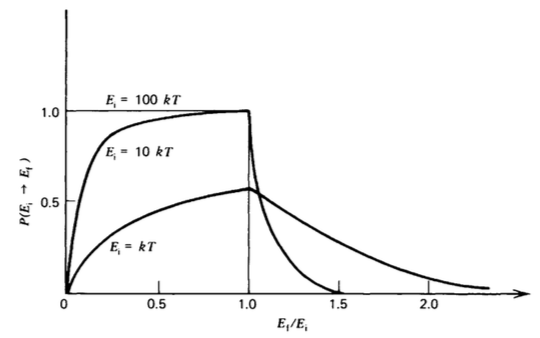
\includegraphics[width=0.5\linewidth]{figures/upscattering.png}
\end{figure}
